%-----------------------------------------------------------------------------%
\chapter{\babSatu}
%-----------------------------------------------------------------------------%
This chapter describes about the background of the research, research questions, research goals, benefits of research, scopes of research, and outline of this thesis proposal.

%-----------------------------------------------------------------------------%
\section{Background}
%-----------------------------------------------------------------------------%
Software is a very essential need for some people or company in this modern era. It is not only used to support a large processes, but also to support the daily activities of its users. Software contains several features which describe the functions of the software. The need for the features could be vary among users. Even for the same type of software, not all features are really needed by the user. That is a challenge for software developers to create software which fits the needs of each users.

Instead of building software from scratch, it will be great if the developers can build software from reusable components. It can reduce the effort of developers to build a software for a user. One concept which relies on building software from reusable components is Software Product Line (SPL) \citep{paper.lee.featuremanagement}.

In Software Product Line (SPL), a software is built from reusable components instead of from scratch so that software development can be done more efficiently \citep{book.apel.FeatureOrientedSoftware}. The software will be built according to the specific needs of each user by using components that are already prepared before. It can reduce the effort of developers in building software for each user. SPL uses the term of {\it feature} to express commonalities and variabilities in software \citep{paper.kastnerApel.FeatureOrientedSoftwareDevelopment}. Features can be functionalities of a software or other software properties. Users can choose which functionalities to be included in their software based on the features provided. Then, the developer can use the reusable components associated with the features to build the software. One language which supports SPL is Abstract Behavioral Specification (ABS).

Abstract Behavioral Specification (ABS) is a modeling language which supports variability by using the concept of SPL \citep{paper.clarke.variability,paper.hanle.ABStutorial,book.abs.abslanguagespecification}. ABS uses feature model to express variability and to organize features \citep{book.abs.abslanguagespecification}. {\it Feature model} is a set of logical constraints that are used to express the dependencies between features. Feature model is represented as a tree of nested features. The example of feature model represented in {\it feature diagram} \citep{paper.kastnerApel.FeatureOrientedSoftwareDevelopment} shown in Figure \ref{fig:FD1}.

\begin{figure}
	\centering
	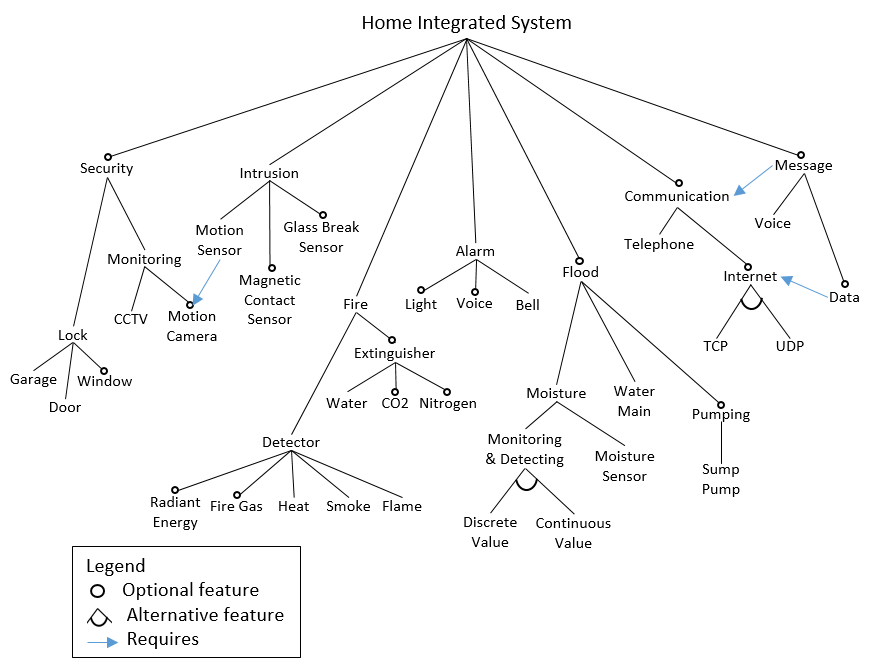
\includegraphics[width=1\textwidth]
		{pics/hisfd4.png}
	\caption{Home Integration System Feature Diagram}
	\label{fig:FD1}
\end{figure}
\vspace{-1cm}
\begin{center}
	{\small Source: \citep{paper.lee.featurebinding} (with additional changes)}
\end{center}

The figure above shows a set of features for Home Integrated System (HIS) \citep{paper.clarke.variability}. There are several features which can be chosen by users, such as {\it Fire, Flood, Alarm, Intrusion}, etc. Some features are general feature which consist of or implemented by the features followed. An {\it Alarm} feature consists of {\it Bell, Voice}, or {\it Light} feature. Then, an {\it Internet} feature implemented by {\it TCP} or {\it UDP} feature. 

A feature model is organized based on the visible characteristics of software \citep{paper.lee.featuremanagement}. It can be very large if the number of features available is also increasing. If a feature model has a large number of features, such as Linux kernel with more than 10.000 features \citep{book.apel.FeatureOrientedSoftware}, it can cause the selection of features process be more complex. To address this problem, the features in the feature model can be grouped based on their functions in general. By grouping the features, the complexity of the feature model can be reduced. Figure \ref{fig:FMGroup1} shows the example of grouped features represented using feature diagram.

\begin{figure}
	\centering
	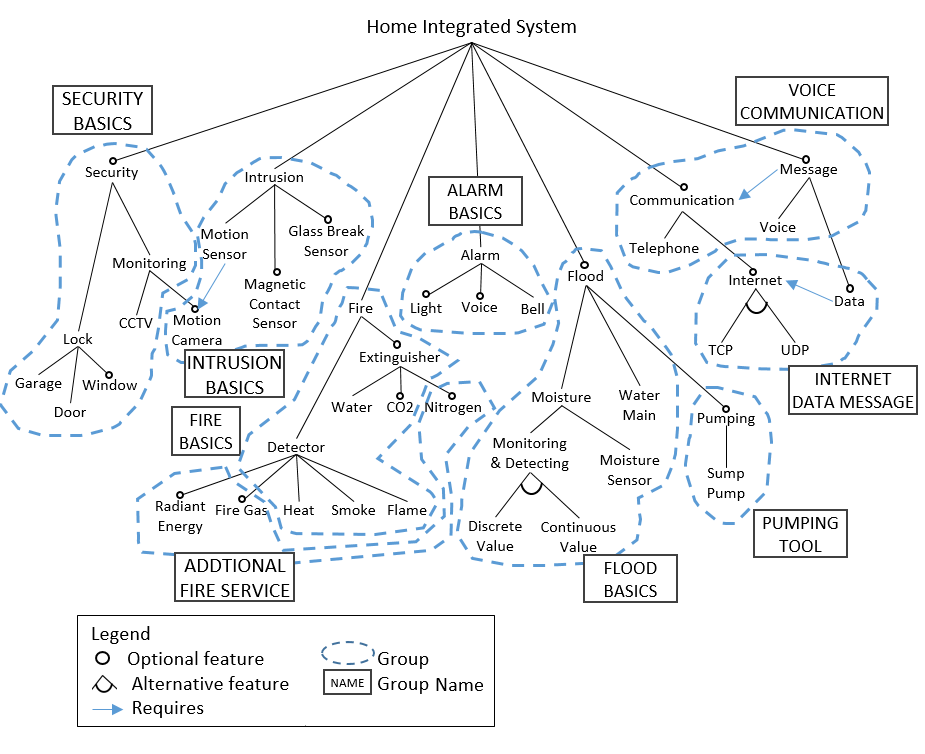
\includegraphics[width=1\textwidth]
	{pics/hisfd4group3.png}
	\caption{Home Integration System Feature Diagram with Grouping}
	\label{fig:FMGroup1}
\end{figure}
\vspace{-1cm}
\begin{center}
	{\small Source: \citep{paper.lee.featurebinding} (with additional changes)}
\end{center}

There are several groups of basic features, as shown on the figure, such as {\it Security Basics, Intrusion Basics, Fire Basics, Flood Basics,} and {\it Alarm Basics}. Moreover, there are features grouped to be additional features, such as {\it Additional Fire Services, Voice Communication, Pumping Tool,} and {\it Internet Data Message}. The features grouped by the common services they provide and the relationship they have. Moreover, the features can be grouped not only by common services they provide, but also by their common domains (e.g. basic or special features for a module), by the target of the users (e.g. small or large companies), and so on.

By now, the selection of features to be included in a software product in ABS is done by listing the features chosen using product selection language (PSL) \citep{paper.hanle.ABStutorial}. It could make the selection of features difficult to do, even more for a user. Thus, the grouped features are intended for the users so they can choose the features easily. As they do not need to see and choose the features based on the feature diagram structure. Moreover, the grouped features need to be made concrete, i.e. visual representation of the grouped features. By using the visual representation of the grouped features, it is expected that the users could choose the features less complex.

In this research the feature grouping mechanism will be made and visualized. The visualization is done by using a simple web application as a tool support. The grouped features and its visualization are intended for users so they can make a selection of features easily. Moreover, the purpose of the feature grouping is to reduce the complexity while doing the features selection. Then, it is expected that the visualization could make the feature selection process more efficient.

Case studies will be used in this research. Those are Charity Organization System (COS) and Odoo Sales module. COS is a system developed to help charity organizations and relies on software product line (SPL) approach and uses ABS language. Odoo Sales module is a part of Odoo software. Odoo is an open-source \citep{web.Odoo.whatIsOdoo,web.Odoo.ERPComparison} enterprise management software \citep{web.Odoo.whatIsOdoo}. COS and Odoo Sales module have features which can be used as the case studies for this research.

%-----------------------------------------------------------------------------%
\section{Research Questions}
%-----------------------------------------------------------------------------%
Based on the research purpose, the research questions which will be answered by this research are as follows:
\begin{enumerate}
	\item {\it How to group the features?}
	Features from feature model or feature diagram need to be grouped. Then, some mechanisms to group the features need to be made.
	
	\item {\it Is the use feature grouping mechanisms to select features better than using the original feature diagram?}
	The feature grouping mechanisms need to be evaluated as those are proposed to make the feature selection process less complex.
	
	\item {\it How grouped feature improve the efficiency of building software?}
	ABS use product selection language as input for generating a software. The grouped feature is intended for the users to choose the features less complex, thus it need to make the process of building the software more efficient.
	
	\item {\it How to make a visualization of the feature grouping?}
	As said on the previous section, the grouped features need to be made concrete (not only abstraction). One to address that is by make a visual representation of those features.
	
	\item {\it How to make the grouping mechanisms and implement them from feature model in ABS tools?}
	Features from feature diagram need to be grouped using some mechanisms. Then, those mechanisms need to be implemented and took the ABS feature model as input.
\end{enumerate}

%-----------------------------------------------------------------------------%
\section{Research Goals}
%-----------------------------------------------------------------------------%
There are several research questions that have been stated. Based on the background of this research and those research questions, there are several goals which will be the target of this research. The research goals are as follows: 
\begin{enumerate}
	\item The feature grouping mechanisms are made to specify how the features should be grouped. 
	
	\item Then, the feature grouping mechanism from feature model in the ABS tools is implemented. Thus, it can generate the feature grouping result from the ABS feature model.The visualization of the result of feature grouping mechanism also need to be implemented. This visualization is expected could be a way to improve the efficiency of building software from the grouped features.
	
	\item Then, the feature grouping mechanisms are evaluated as the result of the research question given.
\end{enumerate}

%-----------------------------------------------------------------------------%
\section{Benefits of Research}
%-----------------------------------------------------------------------------%
Many researchers are contributing in the development of ABS. This research will contribute in the development of ABS because this research goals are to provide the mechanism to group the features and visualize the result.

In practical term, the grouping of features, hopefully, can reduce the complexity while doing the features selection. The visualization of the features selection also gives ease for users to select the features. Then, as stated in the research goals, the visualization could be a way to improve the efficiency of building software from the grouped features.

%-----------------------------------------------------------------------------%
\section{Scope of Research}
%-----------------------------------------------------------------------------%
The aim of this research is to make a grouping mechanism for features and visualize them. To limit the topics discussed in this research, there are scopes of this research as follows:
\begin{enumerate}
	\item The focus of the work is to implement grouping mechanism and the visualization using web application. The grouping mechanism will be implemented in the ABS code generator (compiler back-end). Then, the visualization will be implemented in the web application.
	\item Analyze the grouping mechanism and the visualization using a case study. The case study used is Charity Organization System (COS) and Odoo sales module. The features are taken from COS and Odoo sales module features. For Odoo sales module, several features which are specific to the vendor will be ignored. It is because the ignored features could be not common features in a sales module of an enterprise management software.
\end{enumerate}

%-----------------------------------------------------------------------------%
\section{Outline}
%-----------------------------------------------------------------------------%
The outline of this thesis proposal is describe as follows:
\begin{itemize}
	\item Chapter 1 \babSatu \\
	Chapter 1 describes the introduction of the thesis proposal that includes the background, research questions, research goals and scope, and the systematic of writing.
	\item Chapter 2 \babDua \\
	Chapter 2 contains the literature review and theories which used in this research as the basis to support. This chapter explains software product lines, Abstract Behavioral Specification (ABS), and related works about feature grouping. Additionally, a brief explanation about enterprise software.
	\item Chapter 3 \babTiga \\
	Chapter 3 discuss about the research methodology which consists steps needed to do this research.
	\item Chapter 4 \babEmpat \\
	Chapter 4 explains about the case studies used in this research which are Charity Organization System and Odoo sales module features.
	%\item Chapter 5 \babLima \\
	%\item Chapter 6 \babEnam \\
	%\item Bab 7 \babTujuh \\%
\end{itemize}